\chapter{零知识的属性证明}

在上一章中,我们介绍了如何使用 Sigma 协议来构建身份识别和签名方案。在这些应用中,我们把 Sigma 协议作为``知识证明":利用回溯和知识健全性,我们可以有效地从任何有说服力的证明者那里提取出一个见证。

在本章中,我们将介绍如何使用 Sigma 协议来证明某些事实是真实的(不需要披露太多其他信息)。在以这种方式使用 Sigma 协议的应用中,安全性取决于所谓事实的\emph{真实性},而不是任何\emph{知识}的概念。例如,Chaum-Pedersen 协议(见 \ref{subsec:19-5-2} 小节)允许证明者说服验证者相信一个给定的群元素构成的三元组是一个 DH 三元组。这种能力本身就是构建和分析有趣的加密协议的一个有用工具。

在 \ref{sec:20-1} 节中,我们首先会定义与有效关系相关的\emph{真实陈述的语言}:即存在相应见证的陈述的集合。然后,我们会为 Sigma 协议定义一个\emph{存在健全性}的概念,它意味着任何证明者想要使验证者接受一个不真实的陈述(即不存在对应的见证)是不可行的。这个概念与\emph{知识健全性}不同,因为我们不需要任何种类的见证提取器。然而,我们将会看到,知识健全性本身就意味着存在健全性。

在 \ref{sec:20-2} 节中,我们将提出一系列的例子来说明存在健全性。这些例子围绕着在加密数据上证明属性的想法而展开。

在 \ref{sec:20-3} 节中,然后我们会展示如何使用 Fiat-Shamir 变换(见 \ref{subsec:19-6-1} 小节)的变体将 Sigma 协议变成非交互式证明。

在更后面的章节中,我们将研究构建证明系统的更高级的技术。

\section{语言与存在健全性}\label{sec:20-1}

让我们从一个定义开始。

\begin{definition}[真实陈述的语言]
令 $\mathcal{R}\subseteq\mathcal{X}\times\mathcal{Y}$ 是一个有效关系。如果对于某个 $x\in\mathcal{X}$ 有 $(x,y)\in\mathcal{R}$,那么我们就称陈述 $y\in\mathcal{Y}$ 是一个\textbf{真实陈述 (true statement)},否则称其为\textbf{虚假陈述 (false statement)}。我们称 $L_{\mathcal{R}}$ 为\textbf{由 $\mathcal{R}$ 定义的语言 (language defined by $\mathcal{R}$)},即定义在 $\mathcal{R}$ 上的所有真实陈述,也就是说,$L_{\mathcal{R}}:=\{y\in\mathcal{Y}:(x,y)\in\mathcal{R}\;\text{for some}\;x\in\mathcal{X}\}$。
\end{definition}

上述定义中的``语言 (language)" 一词来自复杂性理论。在本章中,我们将研究一些有趣的关系 $\mathcal{R}$ 以及由它们所定义的语言集合 $L_{\mathcal{R}}$。举一个上一章的例子,回顾一下,Chaum-Pedersen 协议是一个定义在关系
\[
\mathcal{R}:=\bigg\lbrace
\big(\beta, (u,v,w)\big)\in\mathbb{Z}_q\times\mathbb{G}^3:v=g^\beta, w=u^\beta
\bigg\rbrace
\]
上的 Sigma 协议。那么,由 $\mathcal{R}$ 定义的语言 $L_{\mathcal{R}}$ 就是所有 DH 三元组 $(u,v,w)\in\mathbb{G}^3$ 的集合。

于是,我们就可以用下面的攻击游戏来定义存在健全性的概念:

\begin{game}[存在健全性]\label{game:20-1}
令 $\Pi=(P,V)$ 是关系 $\mathcal{R}\subseteq\mathcal{X}\times\mathcal{Y}$ 上的一个 Sigma 协议。对于一个给定对手 $\mathcal{A}$,攻击游戏按照如下方式运行:
\begin{itemize}
	\item 对手 $\mathcal{A}$ 选择一个陈述 $y\in\mathcal{Y}$,并将其发送给挑战者。
	\item 对手 $\mathcal{A}$ 与验证者 $V(y)$ 进行交互,其中挑战者扮演验证者的角色,对手 $\mathcal{A}$ 扮演``作弊的"证明者的角色。
\end{itemize}
如果 $V(y)$ 在交互结束时输出 $\mathsf{accept}$ 但 $y\notin L_{\mathcal{R}}$,我们就称对手 $\mathcal{A}$ 赢得了该游戏。我们定义 $\mathrm{ES}\mathsf{adv}[\mathcal{A},{\Pi}]$ 为对手 $\mathcal{A}$ 对于 $\Pi$ 的优势,其值为对手 $\mathcal{A}$ 赢得该游戏的概率。
\end{game}

\begin{definition}
如果对于所有的有效对手 $\mathcal{A}$,$\mathrm{ES}\mathsf{adv}[\mathcal{A},{\Pi}]$ 的值都可以忽略不计,我们就称 Sigma 协议 $\Pi$ 是\textbf{存在健全 (existentially sound)} 的。
\end{definition}

\begin{theorem}
令 $\Pi$ 是一个有大挑战空间的 Sigma 协议,如果 $\Pi$ 提供知识健全性,那么 $\Pi$ 一定是存在健全的。
\begin{quote}
特别地,对于所有对手 $\mathcal{A}$,我们都有:
\end{quote}
\begin{equation}
\mathrm{ES}\mathsf{adv}[\mathcal{A},{\Pi}]
\leq
\frac{1}{N}
\end{equation}
\begin{quote}
其中 $N$ 是挑战空间的大小。
\end{quote}
\end{theorem}

\begin{proof}
我们只需证明,如果 $\mathcal{A}$ 选择了一个虚假陈述 $y$ 和一个承诺 $t$,那么最多只能有一个挑战 $c$ 使得存在一个应答 $z$ 能够产生一个 $y$ 的接受对话 $(t,c,z)$。观察到,如果有两个这样的挑战,那么 $y$ 将有两个接受对话 $(t,c,z)$ 和 $(t,c',z')$,其中 $c\neq c'$,而知识健全性意味着仅存在一个 $y$ 的见证,这与事实相矛盾。
\end{proof}

我们指出,对于任意强大的对手,上述定理都\emph{无条件}成立。我们在下一节将这些想法付诸实施。
\section{证明加密数据的属性}\label{sec:20-2}

在许多应用中,以下情况都会出现。Alice 用 Bob 的公钥加密一个消息 $m$,得到一个密文 $c$。此外,Alice 想向第三方,比如 Charlie(他可以看到 $c$,但看不到 $m$),证明加密后的明文 $m$ 满足某个属性,但不向 Charlie 透露任何关于 $m$ 的其他信息。

一个存在健全的、特殊 HVZK 的 Sigma 协议可以用来解决这类问题。然而,这样的协议并不是一个完整的解决方案。一个问题是,只有 Charlie 诚实地遵循验证协议时,HVZK 属性才能保证不泄露关于 $m$ 的信息。解决这个问题的一个方法就是使用我们在 \ref{subsec:19-6-1} 小节介绍想法,将交互式识别协议变成签名。也就是说,我们不使用实际的验证者来生成随机挑战,而是使用哈希函数来生成挑战。我们将在下一节中详细介绍这种方法。现在,让我们先来看几个有趣而重要的例子,看看我们如何使用 Sigma 协议来证明加密数据的特定属性。

在我们的例子中,简便起见,我们使用 ElGamal 加密方案的乘法变体,我们曾在练习 11.5 中讨论过。该方案利用由 $g\in\mathbb{G}$ 生成的素阶 $q$ 的循环群 $\mathbb{G}$,私钥是随机选择的 $\alpha\in\mathbb{Z}_q$,公钥是 $u:=g^\alpha\in\mathbb{G}$。明文 $m$ 的加密是 $(v,e)\in\mathbb{G}^2$,其中 $v:=g^\beta$,$e:=u^\beta\cdot m$,并且 $\beta$ 也是从 $\mathbb{Z}_q$ 中随机选取的。要用私钥 $\alpha$ 解密 $(v,e)$,我们需要计算 $m:={e}/{v^\alpha}$。正如我们曾在练习 11.5 中要求的那样,可以证明当 $\mathbb{G}$ 满足 DDH 假设时,上述方案是语义安全的。

\begin{example}[明文相等]
假设 Alice 用 Bob 的公钥 $u_0$ 加密了消息 $m$,得到密文 $(v_0,e_0)$。然后 Alice 又用 Bill 的公钥 $u_1$ 加密了同一个消息 $m$,得到了密文 $(v_1,e_1)$。她想让 Charlie 相信两个密文对应的明文相同,但又不透露任何关于明文的信息。比如说,一些协议可能要求 Alice 向 Bob 和 Bill 广播相同的消息。针对这种场景的协议要求在保持消息加密的同时能够证明 Alice 所加密的明文消息确实是相同的。

因此,所以我们希望有一个关系:
$$
\mathcal{R}:=
\bigg\lbrace
\Big(
(\beta_0,\beta_1,m), (u_0,v_0,e_0,u_1,v_1,e_1)
~\Big) :\\
v_0=g^{\beta_0},\;
e_0=u_0^{\beta_0}\cdot m,\;
v_1=g^{\beta_1},\;
e_1=u_1^{\beta_1}\cdot m\,
\bigg\rbrace
$$
上的 Sigma 协议。语言 $L_\mathcal{R}$ 是元组 $(u_0,v_0,e_0,\,u_1,v_1,e_1)$,使得 $(v_0,e_0)$ 和 $(v_1,e_1)$ 对应在公钥 $u_0$ 和 $u_1$ 下加密的同一消息 $m$。

为了设计一个关系 $\mathcal{R}$ 上的有效 Sigma 协议,我们注意到 $(u_0,v_0,e_0,\,u_1,v_1,e_1)\in L_\mathcal{R}$ 就等价于:
$$
v_0=g^{\beta_0},\;
v_1=g^{\beta_1},\;
{e_0}/{e_1}=u_0^{\beta_0}u_1^{-\beta_1},\ 
\text{ for some }\ \beta_0,\beta_1\in\mathbb{Z}_q
$$

基于这一观察,我们可以使用 \ref{subsec:19-5-3} 小节中介绍的通用线性协议实现一个关系 $\mathcal{R}$ 上的 Sigma 协议。具体来说,Alice 需要向 Charlie 证明存在 $\beta_0$ 和 $\beta_1$ 使得方程组:
$$
v_0 =g^{β_0},\;
v_1=g^{\beta_1},\;
{e_0}/{e_1}=u_0^{\beta_0}u_1^{-\beta_1}
$$
成立。这样就得到了一个关系 $\mathcal{R}$ 上的存在健全的、特殊 HVZK 的 Sigma 协议。

请注意,尽管 Alice 在上述协议中没有显式地使用消息 $m$,但 Alice 还是需要知道它,因为她需要同时知道 $\beta_0$ 和 $\beta_1$,其中任何一个都决定了 $m$。
\end{example}

\begin{example}[明文相等2]
考虑上个例子的一个变体。现在 Alice 有两个密文 $(v_0,e_0)$ 和 $(v_1,e_1)$,这两个密文均来自于 Bob 的公钥 $u$ 所加密的相同的明文。不同的地方在于,现在两个密文均对应着使用\emph{相同}公钥加密的相同明文。同样的,Alice 想要向 Charlie 证明这一事实,但又不向他透露其他信息。注意到,如果 $(v_0,e_0)$ 和 $(v_1,e_1)$ 来自相同的明文,那么:
$$
v_0 =g^{\beta_0},\ 
e_0 =u^{\beta_0}·m,\ 
v_1 =g^{\beta_1},\ 
e_1 =u^{\beta_1}·m
$$
其中 $\beta_0,\beta_1\in\mathbb{Z}_q$,$m\in\mathbb{G}$。用第一式除以第三式,第二式除以第四式,我们可以得到:
\begin{equation}\label{eq:20-2}
{v_0}/{v_1}=g^\beta,\;\;
{e_0}/{e_1}=u^\beta
\end{equation}
其中 $\beta:=\beta_0-\beta_1$。此外,不难看出,如果式 \ref{eq:20-2} 对于某个 $\beta\in\mathbb{Z}_q$ 成立,则 $(v_0,e_0)$ 和 $(v_1,e_1)$ 必然来自对相同明文的加密。

因此,Alice 需要做的就是让 Charlie 相信存在满足式 \ref{eq:20-2} 的 $\beta$。为此,她可以使用 \ref{subsec:19-5-3} 小节介绍的通用线性协议。在本例的场景下,它其实就是证明 $(u,{v_0}/{v_1},{e_0}/{e_1})$ 是一个 DH 三元组的 Chaum-Pedersen 协议(见 \ref{subsec:19-5-2} 小节)。

需要注意的是,为了证明 $(v_0,e_0)$ 和 $(v_1,e_1)$ 加密了相同的消息,Alice 只需要知道满足上式的 $\beta$,她并不需要知道明文消息 $m$ 本身。特别地,Alice 不需要是产生这些密文的一方。事实上,她可以从其他方收到密文 $(v_0,e_0)$,然后通过计算 $v_1:=v_0\cdot g^\beta$ 和 $e_1:=e_0\cdot u^\beta$ 为她选择的 $\beta$ 创建同一消息 $m$ 的新密文 $(v_1,e_1)$。一些匿名服务就能执行类似的功能,他们能够利用这个协议对一个加密消息进行重加密。这个协议可以用来确保这一过程被正确完成。
\end{example}

\begin{example}[加密后的比特]\label{exmp:20-3}
为了加密一个比特 $b\in\{0,1\}$,比较方便的做法是将 $b$ 编码为群元素 $g^b\in\mathbb{G}$,然后用乘性 ElGamal 对 $g^b$ 进行加密。因此,假设 Alice 以这种方式用 Bob 的公钥 $u$ 对比特 $b$ 进行加密,产生一个密文 $(v,e)=(g^\beta,u^\beta\cdot{g^b})$。她想让 Charlie 相信 $(v,e)$ 确实是由 Bob 的公钥加密一个比特得到的(而不是加密其他的什么东西,比如 $g^{17}$),而又不向 Charlie 透露任何其他信息。

因此,我们希望有一个关系:
$$
\mathcal{R}:=
\bigg\lbrace
\Big(
(b,\beta),(u,v,e)
\Big):
v=g^\beta,\;
e=u^\beta\cdot g^b,\;
b\in\{0,1\}\;
\bigg\rbrace
$$
上的 Sigma 协议。与此关系相对应的语言 $L_{\mathcal R}$ 是一个元组 $(u,v,e)$,满足 $(v,e)$ 是用公钥 $u$ 加密一个比特得到的。

我们的 $\mathcal{R}$ 上的 Sigma 协议基于下面的观察,即$(u,v,e)\in L_{\mathcal R}$等价于:
$$
\text{either }
(u,v,e)
\text{ or }
(u,v,{e}/{g})
\text{ is a DH-triple}
$$
\ref{subsec:19-5-2} 中介绍的 Chaum-Pedersen 协议允许一方证明一个给定的三元组是 DH 三元组。我们把它与 \ref{subsec:19-7-2} 中介绍的 OR 证明构造结合起来。这为我们提供了一个关系:
$$
\mathcal{R}':=
\bigg\lbrace
\Big(
(b,\beta),\;((u_0,v_0,w_0),\;(u_1,v_1,w_1))
\Big):
v_b=g^\beta,~
w_b=u_b^\beta\;
\bigg\rbrace
$$
上的 Sigma 协议。如果 $(u_0,v_0,w_0)$,$(u_1,v_1,w_1)$ 中至少有一个是 DH 三元组,则语句 $((u_0,v_0,w_0),(u_1,v_1,w_1))$ 就在 $L_{\mathcal{R}'}$ 中。于是,我们有:
$$
(u,v,e)\in L_{\mathcal R}\ \iff\ 
\Big((u,v,e),(u,v,{e}/{g})\Big)\in L_{\mathcal R'}
$$
因此,为了让 Alice 向 Charlie 证明 $(u,v,e)\in L_{\mathcal{R}}$,可以使用陈述 $((u,v,e),(u,v,{e}/{g}))$ 和见证 $(b,\beta)$ 运行一个 $\mathcal{R}'$ 上的 Sigma 协议。完整起见,我们在图 \ref{fig:20-1} 中展示了完整的 $\mathcal R$ 上的 Sigma 协议。在证明者逻辑的第一行,证明者为其知道的见证启动证明过程,第二和第三行为其不知道的见证运行 HVZK 模拟器。由此产生的 $\mathcal R$ 上的 Sigma 协议是存在健全的,并且是特殊 HVZK 的。

\begin{figure}
  \centering
  \includegraphics[width=0.85\linewidth]{figures/chapter20/fig1.png}
  \caption{用于加密比特的 Sigma 协议}
  \label{fig:20-1}
\end{figure}

正如练习 20.6 将要说明的,该协议可以泛化为证明一个密文 $(v,e)$ 在 $B>2$ 的情况下加密了一个值 $0\leq b < B$。该协议的交互记录随 $B$ 的增大线性增长,因此只适用于相对较小的 $B$。我们会在 \ref{subsec:20-4-1} 小节介绍如何处理 $B$ 较大的情况。
\end{example}

\begin{example}[加密后的 DH 三元组]\label{exmp:20-4}
假设 Alice 有一个 DH 三元组 $(g^{\gamma_1},g^{\gamma_2},g^{\gamma_3})$,其中 $\gamma_3=\gamma_1\gamma_2$。她使用 Bob 的公钥 $u$ 对每个元素进行加密,生成了三条密文 $(v_1,e_1)$,$(v_2,e_2)$,$(v_3,e_3)$,其中:
\begin{equation}\label{eq:20-3}
v_i=g^{\beta_i},\;
e_i=u^{\beta_i}g^{\gamma_i}\;\;
(i = 1,2,3)
\end{equation}
她把这些密文交给 Charlie,并想让他相信这些密文确实是对一个 DH 三元组的加密,但又不透露任何其他信息。

因此,我们希望有一个关系:
$$
\mathcal R:=
\bigg\lbrace
\Big((\beta_1,\beta_2,\beta_3,\gamma_1,\gamma_2,\gamma_3),(u,v_1,e_1,v_2,e_2,v_3,e_3)\Big):\\
v_i=g^{\beta_i},\;
e_i=u^{\beta_i}g^{\gamma_i}\,(i=1,2,3),\;
\gamma_3=\gamma_1\gamma2
\bigg\rbrace
$$
上的 Sigma 协议。相应的语言 $L_{\mathcal R}$ 是满足密文 $(v_1,e_1)$,$(v_2,e_2)$,$(v_3,e_3)$ 是由公钥 $u$ 加密一个 DH 三元组得到的元组 $(u,\;v_1,e_1,\;v_2,e_2,\;v_3,e_3)$。

虽然由于条件 $\gamma_3=\gamma_1\gamma_2$,关系 $\mathcal R$ 本质上是非线性的,但我们还是可以使用 \ref{subsec:19-5-3} 中介绍的通用线性协议为 $\mathcal R$ 设计一个 Sigma 协议。其基本思想是,Alice 向 Charlie 证明,存在$\beta_1$、$\beta_3$、$\gamma_1$ 和 $\tau$满足方程组:
\begin{equation}\label{eq:20-4}
v_1=g^{\beta_1},~~
e_1=u^{\beta_1}g^{\gamma_1},~~
v_3=g^{\beta_3},~~
v_2^{\gamma_1}=g^\tau,~~
e^{\gamma_1}u^{\beta_3}=e_3u^\tau
\end{equation}

为了证明这一点,我们声称 $(u,v_1,e_1,v_2,e_2,v_3,e_3)\in L_{\mathcal R}$ 成立当且仅当存在能够满足式 \ref{eq:20-4} 的 $\beta_1,\beta_3,\gamma_1,\tau$。注意到,密文 $(v_1,e_1)$,$(v_2,e_2)$,$(v_3,e_3)$ 唯一决定了 $\beta_i$ 和满足式 \ref{eq:20-3} 的 $\gamma_i$。$\beta_1$,$\beta_3$ 和 $\gamma_1$ 也是满足式 \ref{eq:20-4} 中前三个等式的唯一值。式 \ref{eq:20-4} 中的第四个方程可以通过令 $\tau:=\gamma_1\beta_2$ 而得到唯一的满足。因此,剩下的工作就是考虑式 \ref{eq:20-4} 中最后一个方程,其等号左边为:
$$
e^{\gamma_1}u^{\beta_3}=(u^{\beta_2}g^{\gamma_2})^{\gamma_1}u^{\beta_3}=u^{\beta_3+\tau}g^{\gamma_1\gamma_2}
$$
而等号右边为:
$$
e_3u^\tau=(u^{\beta_3}g^{\gamma_3})u^\tau =u^{\beta_3+\tau}g^{\gamma_3}
$$
因此,当且仅当 $\gamma_1\gamma_2=\gamma_3$ 时,该方程成立。这就证明了我们的声称。

这样,我们就得到了 $\mathcal R$ 上的 Sigma 协议。为了运行该协议,Alice 使用见证 $(\beta_1,\beta_3,\gamma_1,\tau:= \gamma_1\beta_2)$ 运行式 \ref{eq:20-4} 的通用线性协议。该协议的正确性、存在健全性和特殊 HVZK 性都来自于通用线性协议的相应属性。
\end{example}

\begin{example}[加密后的比特 2]\label{exmp:20-5}
利用上一个例子的思路,我们可以得到用于例 \ref{exmp:20-3} 中加密比特问题的另一个 Sigma 协议。

如果 Alice 想向 Charlie 证明密文 $(v,e)$ 形如 $v=g^\beta$,$e=u^\beta g^b$,其中 $b=\{0,1\}$,她只需要说明 $b^2=b$,因为 $b\in\mathbb{Z}_q$ 中满足 $b^2=b$ 的就只有 $b=0$ 或者 $b=1$。

因此,使用通用线性协议,Alice 只要向 Charlie 证明存在 $b,\beta,\tau(=\beta b)$ 满足方程组:
$$
v=g^\beta,~~
e=u^\beta g^b,~~
v^b=g^\tau,~~
e^b=u^\tau g^b
$$
读者可以自行验证这是否能够产生针对例 \ref{exmp:20-3} 中关系 $\mathcal R$ 的一个存在健全的、特殊 HVZK 的 Sigma 协议。所得到的协议与例 \ref{exmp:20-3} 中的加密比特协议具有类似的性能表现。

这个协议可以推广到向 Charlie 证明,一个密文 $(v,e)$ 来自对值 $0\leq b < B$ 的加密,其中 $B>2$。这种推广使用到了下一个例子中将要介绍的 Sigma 协议,用于向 Charlie 证明 $b$ 满足多项式关系$b(b-1)(b-2)\cdots(b-(B-1))=0$。该关系意味着 $0\leq b < B$。该协议的交互记录同样随 $B$ 的增大而线性增长,因此也只适用于相对较小的 $B$。
\end{example}

\begin{example}[多项式关系]\label{exmp:20-6}
我们可以进一步扩展例 \ref{exmp:20-4} 的想法。假设 Alice 用 Bob 的公钥 $u$ 生成两个密文 $(v,e)$ 和 $(v',e')$,第一个密文来自对群元素 $g^\gamma$ 的加密,第二个则来自 $g^{\gamma'}$。Alice 想让 Charlie 相信,对于某个特定的多项式 $f(x)=\sum_{i=0}^d\lambda_ix^i$,有 $\gamma'=f(\gamma)$。我们将假设多项式 $f(x)$ 的阶 $d$ 和系数 $\lambda_0,\dots,\lambda_d$ 都是固定且公开的值(即为常数或者系统参数)。

因此,我们想要一个关系:
$$
\mathcal R=
\bigg\lbrace
\Big((\beta,\gamma,\beta',\gamma'),(u,v,e,v',e')\Big):
v=g^\beta,\;
e=u^\beta\cdot g^\gamma,\;
v'=g^{\beta'},\;
e'=u^{\beta'}\cdot g^{\gamma'},\;
\gamma'=f(\gamma)
\bigg\rbrace
$$
上的 Sigma 协议。

为了得到 $\mathcal R$ 上的 Sigma 协议,Alice 和 Charlie 使用通用线性协议,其中 Alice 向 Charlie 证明,存在:
$$
\beta,~~~
\gamma_1,\dots,\gamma_d,~~~
\tau_1,\dots,\tau_{d-1},~~~
\beta',~
\gamma'
$$
满足方程组:
\begin{equation*}
\begin{aligned}
& v=g^\beta,\;
e=u^\beta g^{\gamma_1},\;
v'=g^{\beta'},\;
e'=u^{\beta'}g^{\gamma'},\;
\gamma'=\lambda_0+\lambda_1\gamma_1+\cdots+\lambda_d\gamma_d,\\
& v^{\gamma_i}=g^{\tau_i},\;
e^{\gamma_i}=u^{\tau_i}g^{\gamma_{i+1}}\;\;\;
(i=1,\dots,d-1)
\end{aligned}
\end{equation*}
请注意,这里我们使用的是通用线性协议的推广版本,它能够处理 $\mathbb G$ 和 $\mathbb{Z}_q$ 上的方程(见定理 \ref{theo:19-11} 之后的讨论)。Alice 使用 $\gamma_i:=\gamma^i,~~i=1,\dots,d$ 和 $\tau_i:=\beta\gamma^i,~~i=1,\dots,d-1$ 运行该协议。读者可以证明,这些实际上是满足这个方程组的唯一取值。通过一个简单的归纳论证可以很容易地证明这一点。由此可见,所得到的 Sigma 协议是一个关系 $\mathcal R$ 上存在健全的,特殊 HVZK 的Sigma 协议。
\end{example}

以上的例子展示了\emph{语言规约}的概念。一般来说,这种从 $\mathcal{R}\subseteq\mathcal{X}\times\mathcal{Y}$ 到 $\mathcal{R}'\subseteq\mathcal{X}'\times\mathcal{Y}'$ 的规约是一对可有效计算的映射 $f:\mathcal{X}\times\mathcal{Y}\to\mathcal{X}'$ 和 $g:\mathcal{Y}\to\mathcal{Y}'$,使得:
\begin{enumerate}[(i)]
	\item 对于所有 $(x,y)\in\mathcal{R}$ 都有 $(f(x,y),g(y))\in\mathcal{R}'$ 成立,并且
	\item 对于所有 $y\in\mathcal{Y}$,$g(y)\in L_{\mathcal{R}'}\; \Longrightarrow\; y\in L_{\mathcal R}$。
\end{enumerate}
利用这样的规约,我们就可以利用 $\mathcal{R}'$ 上的 Sigma 协议 $\Pi'$ 来构造一个 $\mathcal{R}$ 上的 Sigma 协议 $\Pi$。上面的第一个条件能够确保 $\Pi$ 能够从 $\Pi'$ 处继承正确性和特殊 HVZK 性,第二个条件确保 $\Pi$ 能够从 $\Pi'$ 处继承存在健全性。注意,知识可靠性不一定需要继承。也就是说,我们不要求可以从 $g(y)$ 的见证中恢复 $y$ 的见证。在上述几乎所有的例子中,关系 $\mathcal{R}'$ 都是通用线性关系的特例。唯一的例外是例 \ref{exmp:20-3},其关系 $\mathcal{R}'$ 来自 OR 证明构造。

\subsection{一种用于非线性关系的通用协议}\label{subsec:20-2-1}

在上面的几个例子中,我们可以看到,通用线性协议可以用于证明某些非线性关系。我们下面将展示更加通用的情况。正如我们将要看到的,例 \ref{exmp:20-6} 中的多项式求值协议可以很容易地推导出这种构造的一个特例。同样的通用构造也可以用来推导出针对例 \ref{exmp:20-4} 和例 \ref{exmp:20-4} 中的问题的协议;然而,所得到的协议不会像这两个例子中的协议那样高效。

与往常一样,令 $\mathbb{G}$ 是一个由 $g\in\mathbb{G}$ 生成的素阶 $q$ 的循环群。考虑 \ref{subsec:19-5-3} 小节中介绍的通用线性协议,该协议适用于形如式 \ref{eq:19-13} 所描述的公式 $\phi$。假设我们现在也允许 $\phi$ 中存在形如 $x_i=x_j\cdot x_k$ 的非线性方程。为了这个构造仍然有效,我们要求对于每个这样的非线性方程,$\phi$ 中还需要包含形如下面这样的两个辅助方程:
\begin{equation}\label{eq:20-5}
v=g^{x_\ell},\;\;
e=u^{x_\ell}g^{x_j}
\end{equation}
其中 $u$,$v$ 和 $e$ 都是群 $\mathbb{G}$ 中的元素,而 $x_\ell$ 是某个变量。为了简单起见,我们假设在对 $\phi$ 的描述中,存在从每个非线性方程到对应辅助方程的指针。

我们可以将这样的公式 $\phi$ 转化为可以使用通用线性协议处理的方程 $\phi'$,方法如下。对于 $\phi$ 中的每个非线性方程 $x_i=x_j\cdot x_k$ 以及式 \ref{eq:20-5} 中相应的辅助方程,我们引入一个临时变量 $t$,并将非线性方程 $x_i=x_j\cdot x_k$ 替换为下面的一对方程:
\begin{equation}\label{eq:20-6}
v^{x_k}=g^t,~~
e^{x_t}=u^th^{x_i}
\end{equation}

这种变换的结果就是一个可以用通用线性协议处理的方程 $\phi'$。用于 $\phi$ 的 Sigma 协议的工作原理如下。证明者和验证者都可以将 $\phi$ 转化为 $\phi'$。假设证明者有变量 $(x_1,\dots,x_n)$ 的一个赋值 $(\alpha_1,\dots,\alpha_n)$,该赋值能够使得 $\phi$ 的值为 $\mathsf{true}$。那么对于 $\phi$ 中的每个非线性方程 $x_i=x_j\cdot x_k$,证明者为式 \ref{eq:20-6} 中的临时变量 $t$ 赋值 $\alpha_k\alpha_\ell$,然后用这个扩展赋值与验证者一起运行 $\phi'$ 的通用线性协议。

读者可以验证,这种变换得到的 Sigma 协议是特殊 HVZK 的,并且为关系 \ref{eq:19-14} 提供知识健全性,其中方程 $\phi$ 现在被允许具有上述的非线性形式。

\begin{snote}[多项式计算.]
例 \ref{exmp:20-6} 中的协议可以用这种转换方式导出。Alice 向 Charlie 证明,存在:
$$
\beta,~~
\gamma_1,\dots,\gamma_d,~~
\beta',~
\gamma'
$$
满足方程组:
\begin{equation*}
\begin{aligned}
& v=g^\beta,~~
e=u^\beta g^{\gamma_1},~~
v'=g^{\beta'},~~
e'=u^{\beta'}g^{\gamma'},~~
\gamma'=\lambda_0+\lambda_1\gamma_1+\cdots+\lambda_d\gamma_d,\\
& \gamma_{i+1}=\gamma_1\cdot\gamma_i~~~(i=1,\dots,d-1)
\end{aligned}
\end{equation*}
读者可以自行验证,从非线性到线性的变换能够将每个方程 $\gamma_{i+1}=\gamma_1\cdot\gamma_i$ 转换为一对方程 $v^{\gamma_i}=g^{\tau_i}$ 和 $e^{\gamma_i}=u^{\tau_i}g^{\gamma_{i+1}}$。
\end{snote}

\begin{snote}[加密后的比特.]
例 \ref{exmp:20-5} 中的协议也可以用这种变换得出。Alice 向 Charlie 证明存在 $b$ 和 $\beta$ 使得:
$$
v=g^\beta,\;
e=u^\beta g^b,\;
b=b\cdot b
$$
成立。读者可以自行证明,从非线性到线性的变换能够得出例 \ref{exmp:20-5} 中的协议。
\end{snote}

\begin{snote}[加密后的 DH 三元组.]

我们也可以尝试使用这种技术来设计例 \ref{exmp:20-4} 中的协议。最明显的方法是让 Alice 向 Charlie 证明,存在:
$$
\beta_1,\beta_2,\beta_3,~~~~
\gamma_1,\gamma_2,\gamma_3
$$
使得:
$$
v_i=g^{\beta_i},\;
e_i=u^{\beta_i}g^{\gamma_i}~~(i=1,2,3),\;
\gamma_3=\gamma_1\gamma_2
$$
成立。我们可以将这个方程组插入上述从非线性到线性的变换中。这样做是可行的,但得到的协议不会像例 \ref{exmp:20-4} 中的协议那样高效。
\end{snote}

\begin{snote}[去除对非线性方程的约束.]
虽然我们的通用变换相当有用,但它仍然受到一定的限制。事实上,我们要求对于每个非线性方程 $x_i=x_j\cdot x_k$,方程组还必须包括描述使用乘性 ElGamal 加密 $x_j$ 或 $x_k$ 的方程。稍后,在 \ref{subsec:20-4-3} 小节中,我们将看到,如果我们愿意使用相对较弱(但仍然有用)的 HVZK 形式(或较弱的知识健全性形式,见练习 20.5),我们就可以去掉这一要求。
\end{snote}
\section{非交互式证明系统}\label{sec:20-3}

在上一节中,我们介绍了存在健全的 Sigma 协议的概念。在这一节中,我们将展示如何使用 Fiat-Shamir 变换(见 \ref{subsec:19-6-1} 小节)将任意 Sigma 协议转换为一个\emph{非交互式证明系统}。

基本思想非常简单:我们不依靠验证者来生成随机挑战,而是使用哈希函数 $H$ 从陈述和承诺中推导出挑战。如果将 $H$ 建模为一个随机预言机,那么我们可以证明以下事实:
\begin{enumerate}[(i)]
	\item 如果 Sigma 协议是存在健全的,那么导出的非交互式证明系统也是存在健全的;
	\item 如果 Sigma 协议是特殊 HVZK 的,那么运行对应的非交互式证明系统不会透露关于证明者的见证的任何有用信息。
\end{enumerate}

第一个属性是对存在健全性概念在非交互式环境中的一个相当直接的应用。第二个属性是一个新型的``零知识"属性,定义起来可能有点棘手。

\subsection{例子:一个投票协议}

在给出正式定义之前,我们先通过展示一个投票协议来说明非交互式协议的功能。对投票协议进行正确建模需要相当大的努力,光是全面考虑安全要求就相当具有挑战性,我们不会在这里尝试这样做。相反,我们只会简要阐述基本的想法,并对其他的问题给出简单的提示。

现在假设我们有 $n$ 个投票者,每个投票者都可以投 $0$ 或 $1$ 的票。在投票结束时,所有各方都应该知道票数的总和。当然,每个投票者都可以直接公布他们的投票内容。但是这并不是一个很好的解决方案,因为我们希望允许投票者保有他们的隐私。为此,一些投票协议会使用加密方案,使每个投票者公布其投票的加密信息。

一个方便的方案是 ElGamal 方案的乘性变体,我们已经在 \ref{sec:20-2} 节讨论过部分内容。同样,我们现在有一个由 $g\in\mathbb{G}$ 生成的素阶 $q$ 的循环群 $\mathbb{G}$。私钥 $\alpha\in\mathbb{Z}_q$,公钥 $u:=g^\alpha\in\mathbb{G}$。对消息 $m\in\mathbb{G}$ 的加密能得到 $(v,e)$,其中 $v:=g^\beta$,$e:=u^\beta\cdot m$。

我们下面介绍的设计是一个简单的尝试,它能够在一定程度上保护投票者的隐私。假设我们有一个可信服务器,称为\emph{投票统计中心}(VTC),它能够运行密钥生成算法并获得一个公钥 $pk=u$ 和一个私钥 $sk=\alpha$。它向所有投票者公布 $pk$,然后自己保留 $sk$。

\emph{投票阶段。}
在投票阶段,第 $i$ 个投票者将它的投票 $b_i\in\{0,1\}$ 加密,即将 $b_i$ 编码为群元素 $g^{b_i}\in\mathbb{G}$,然后用 VTC 的公钥对 $g^{b_i}$ 进行加密,得到密文 $(v_i,e_i)$。注意 $v_i=g^{\beta_i}$,$e_i=u^{\beta_i}\cdot g^{b_i}$,其中 $\beta_i\in\mathbb{Z}_q$ 是随机选出的。所有密文都会被公开。

\emph{计票阶段。}
VTC 将所有公布的密文聚合为一个单一的密文 $(v_*,e_*)$,其中:    
$$
v_*:=\prod_{i=1}^nv_i,~~
e_*:=\prod_{i=1}^ne_i
$$
令 $\beta_*:=\sum_i\beta_i$,$\sigma:=\sum_ib_i$,则有:
$$
v_*=g^{\beta_*},~~
e_*=u^{\beta_*}g^\sigma
$$
因此,$(v_*,e_*)$ 就相当于对 $g^\sigma$ 的加密。所以,VTC 可以解密 $(v_*,e_*)$ 并公布结果,这样所有投票者就都可以看到 $g^\sigma$。由于 $\sigma$ 本身是一个小数字,所以不难从 $g^\sigma$ 还原出 $\sigma$,只要通过暴力搜索或查表就可以了。

如果所有的投票者和 VTC 都正确地遵守协议,那么至少从直观上看,ElGamal 加密的语义安全能够确保在投票阶段结束时没有任何一个投票者能知道其他人的投票内容。此外,在计票阶段结束时,任何一个投票者都只能知道票数的总和,没有关于任何单独选票的额外信息会被披露。

上述协议不是很健壮,因为如果任何一个投票者或 VTC 被攻陷,选举结果的正确性和投票内容的隐私都可能受到影响。目前,我们先继续假设 VTC 是诚实的(本章后的一些练习会讨论防止 VTC 作弊的思路)。相对地,让我们把重点放在投票者作弊的可能性上。

投票者作弊的一种方式是将 $0$ 或 $1$ 以外的内容作为投票进行加密。比如说,它可能加密的并不是 $g^0$ 或者 $g^1$,而是 $g^{100}$。这就相当于它投了 $100$ 张内容为 $1$ 的票,这将使投票者能够不公平地影响选举的结果。

为了防止这种情况,当一个投票者投票时,我们应该坚持要求它\emph{证明}其加密的投票 $(v_i,e_i)$ 是\emph{有效的},即它形如 $(g^\beta,u^\beta\cdot g^b)$,其中 $b\in\{0,1\}$。为了做到这一点,我们对例 \ref{exmp:20-3} 中的 Sigma 协议应用 Fiat-Shamir 变换。投票者(使用见证 $(b,\beta)$)只需运行图 \ref{fig:20-1} 中证明者的逻辑,通过计算陈述和承诺的哈希来自行生成挑战。在此例中为:
\begin{equation}\label{eq:20-7}
c\leftarrow H(\;(u,v,e),\;(v_{\rm t0},w_{\rm t0},v_{\rm t1},w_{\rm t1})\;)
\end{equation}
投票者随后公布证明:
\begin{equation}\label{eq:20-8}
\pi=(\;(v_{\rm t0},w_{\rm t0},v_{\rm t1},w_{\rm t1}),\;(c_0,\beta_{\rm z0},\beta_{\rm z1})\;)
\end{equation}
和密文 $(v,e)$。任何人(特别是 VTC)都可以检查证明 $\pi$ 的合法性,即检查 $\pi$ 是否满足图 \ref{fig:20-1} 中验证者会验证的相应条件,区别只是现在 $c$ 是由哈希函数 $H$ 计算出来的,如式 \ref{eq:20-7}。

正如我们将看到的,如果我们把哈希函数 $H$ 建模为一个随机预言机,那么该证明就是健全的。也就是说,如果加密后的投票无效,那么构造出一个合法的证明在计算上是不可行的。此外,零知识属性将确保证明本身不会泄露任何关于投票内容的额外信息。事实上,如果我们定义一个新的、增强的加密方案,其中密文的形式为 $(v,e,\pi)$,那么我们可以证明这个增强的加密方案是语义安全的(在DDH假设下,$H$被建模为一个随机预言机)。我们把这个问题留给读者作为练习。

我们可以按照 \ref{subsec:19-2-3} 小节介绍的优化 Schnorr 签名的思路来优化这个证明系统。也就是说,我们可以使用形如:
$$
\pi^*=(c_0,c_1,\beta_{\rm z0},\beta_{\rm z1})
$$
的证明来代替式 \ref{eq:20-8} 中的证明 $\pi$。

为了验证该证明,我们可以从验证方程中推导出 $v_{\rm t0},w_{\rm t0},v_{\rm t1},w_{\rm t1}$ 的值(即计算 $v_{\rm t0}\leftarrow{g^{\beta_{\rm z0}}}/{v^{c_0}}$,以此类推),然后检查 $c_0\oplus c_1=H((u,v,e),(v_{\rm t0},w_{\rm t0},v_{\rm t1},w_{\rm t1}))$ 是否成立。在实践中,人们会使用这个优化后的系统,因为其证明更加紧凑,并且提供与未优化系统相同的安全属性(包括健全性和零知识性)。读者可参见练习 20.14 以了解这类优化可能存在的更多一般条件。练习 20.26 探讨了如何加强这个投票协议以对抗恶意的 VTC。

\subsection{非交互式证明:基本语法}

下面我们开始着手定义非交互式证明的一般情况及其安全属性,以及 Fiat-Shamir 变换的细节。

我们首先定义非交互式证明的基本语法。

\begin{definition}[非交互式证明系统]
令 $\mathcal{R}\subseteq\mathcal{X}\times\mathcal{Y}$ 是一个有效关系。\textbf{$\mathcal R$ 上的非交互式证明系统 (non-interactive proof system for $\mathcal{R}$)} 是一对算法 $(Gen,Check)$,其中:
\begin{itemize}
	\item $Gen$ 是一个有效概率性算法,它的调用方式为 $\pi\overset{\rm R}\leftarrow Gen(x,y)$,其中 $(x, y)\in\mathcal{R}$,并且 $\pi$ 属于某个\textbf{证明空间 (proof space)} $\mathcal{PS}$;
	\item $Check$ 是一个有效确定性算法,它的调用方式为 $Check(y,\pi)$,其中 $y\in\mathcal{Y}$,$\pi\in\mathcal{PS}$。$Check$ 的输出为 $\mathsf{accept}$ 或 $\mathsf{reject}$。如果 $Check(y,\pi)=\mathsf{accept}$,我们就称 \textbf{$\pi$ 是 $y$ 的一个有效证明 (a valid proof for $y$)}。
\end{itemize}
我们要求对于所有 $(x, y)\in\mathcal{R}$,$Gen(x,y)$ 的输出总是 $y$ 的有效证明。
\end{definition}

\subsection{Fiat-Shamir 变换}

我们下面详细介绍将 Sigma 协议转换为非交互式证明系统的 Fiat-Shamir 变换。

令 $\Pi=(P,V)$ 是一个关系 $\mathcal{R}\subseteq\mathcal{X}\times\mathcal{Y}$ 上的 Sigma 协议。假设 $\Pi$ 的对话 $(t,c,z)$ 属于 $\mathcal{T}\times\mathcal{C}\times\mathcal{Z}$。令 $H:\mathcal{Y}\times\mathcal{T}\to\mathcal{C}$ 是一个哈希函数。我们定义 Fiat-Shamir 非交互式证明系统 ${\rm FS}\text{-}\Pi=(Gen,Check)$,其验证空间 $\mathcal{PS}=\mathcal{T}\times\mathcal{Z}$,如下所示:
\begin{itemize}
	\item 对于输入 $(x,y)\in\mathcal{R}$,$Gen$ 首先运行 $P(x,y)$ 以获得承诺 $t\in\mathcal{T}$,然后将挑战 $c:=H(y,t)$ 转发给 $P(x,y)$ 获得应答 $z\in\mathcal{Z}$。$Gen$ 的输出为 $(t,z)\in\mathcal{T}\times\mathcal{Z}$;
	\item 对于输入 $(y,(t,z))\in\mathcal{Y}\times(\mathcal{T}\times\mathcal{Z})$,$Check$ 验证 $(t,c,z)$ 是否是 $y$ 的一个接受对话,其中 $c:=H(y,t)$。
\end{itemize}

\subsection{非交互式存在健全性}

我们接下来把存在健全性的定义应用到非交互式的环境中。从本质上说,该定义指为一个错误的陈述制造一个有效证明是很难的。

\begin{game}[非交互式存在健全性]\label{game:20-2}
令 $\Phi=(Gen,Check)$ 是 $\mathcal{R}\subseteq\mathcal{X}\times\mathcal{Y}$ 上的一个非交互式证明系统,其证明空间为 $\mathcal{PS}$。为了攻击 $\Phi$,对抗者 $\mathcal{A}$ 输出一个陈述 $y\in\mathcal{Y}$ 和一个证明 $\pi\in\mathcal{PS}$。

如果 $Check(y,\pi)=\mathsf{accept}$ 但 $y\notin L_{\mathcal R}$,我们就称对手 $\mathcal A$ 赢得游戏。我们将 $\mathcal{A}$ 相对于 $\Phi$ 的优势记为 ${\rm niES\mathsf{adv}}[\mathcal{A},\Phi]$,其值为 $\mathcal{A}$ 赢得该游戏的概率。
\end{game}

\begin{definition}
如果对所有有效对手 $\mathcal{A}$,${\rm niES\mathsf{adv}}[\mathcal{A},\Phi]$ 的值都可忽略不计,我们就称 $\Phi$ 是\textbf{存在健全的 (existential sound)}。
\end{definition}

我们下面会说明,在适当的假设下,如果我们将哈希函数建模为随机预言机,那么 Fiat-Shamir 变换可以导出一个存在健全的非交互式证明系统。

\begin{theorem}
设 $\Pi$ 是关系 $\mathcal{R}\subseteq\mathcal{X}\times\mathcal{Y}$ 上的一个 Sigma 协议,令 ${\rm FS}\text{-}\Pi$ 是由 $\Pi$ 派生的带有哈希函数 $H$ 的 Fiat-Shamir 非交互式证明系统,如果 $\Pi$ 是存在健全的,且 $H$ 被建模为一个随机预言机,那么 ${\rm FS}\text{-}\Pi$ 是存在健全的。
\begin{quote}
特别地,令 $\mathcal{A}$ 是攻击游戏 \ref{game:20-2} 的随机预言机版本中攻击 ${\rm FS}\text{-}\Pi$ 健全性的对手。此外,假设 $\mathcal{A}$ 最多发出 $Q_{\rm ro}$ 次随机预言机查询。那么必然存在一个攻击游戏 \ref{game:20-1} 中攻击 $\Pi$ 存在健全性的对手 $\mathcal{B}$,其中 $\mathcal{B}$ 是 $\mathcal{A}$ 的一个基本包装器,使得:
\end{quote}
$$
{\rm niES^{ro}\mathsf{adv}}[\mathcal{A},{\rm FS}_\Pi]\leq(Q_{\rm ro}+1)\cdot{\rm ES\mathsf{adv}}[\mathcal{B},\Pi]
$$
\end{theorem}

\begin{proof}[证明简述]
基本思想类似于我们在证明 Schnorr 签名方案的安全性时的分析(见定理 \ref{theo:19-7})。假设 $\mathcal{A}$ 在一个错误的陈述 $y$ 上产生一个有效的证明 $(t,z)$,这意味着 $(t,c,z)$ 是 $y$ 的一个有效对话,其中 $c$ 是随机预言机在 $(y,t)$ 点的输出。不失一般性,我们可以假设 $\mathcal{A}$ 在这一点上查询了随机预言机(即使它没有这样做,我们也可以使其如此,即把随机预言机的查询次数增加到 $Q_{\rm ro}+1$)。然后,我们的对手 $\mathcal{B}$ 开始(预先)猜测 $\mathcal{A}$ 的随机预言机查询中的哪一个将是相关的。在 $\mathcal{A}$ 进行随机预言机查询的时候,$\mathcal{B}$ 向自己的挑战者发起证明尝试,提供 $y$ 作为陈述,$t$ 作为承诺;$\mathcal{B}$ 的挑战者则以一个随机挑战 $c$ 作为应答,$\mathcal{B}$ 将其转发给 $\mathcal{A}$,就好像它就是 $(y,t)$ 处随机预言机的值。如果 $\mathcal{B}$ 的猜测是正确的,那么 $\mathcal{A}$ 的证明中的值 $z$ 将让 $\mathcal{B}$ 在它的攻击游戏中获胜。安全约束中存在因子 $(Q_{\rm ro}+1)$ 是由于 $\mathcal{B}$ 猜中的概率恰好为 ${1}/{(Q_{\rm ro}+1)}$。
\end{proof}

\subsection{非交互式零知识}

令 $\Phi=(Gen,Check)$ 是关系 $\mathcal{R}\subseteq\mathcal{X}\times\mathcal{Y}$ 上的一个非交互式证明系统,其证明空间为 $\mathcal{PS}$。我们希望定义一个有用的``零知识"的概念。直观地讲,我们希望这个概念能够反映出这样的想法,即 $Gen$ 在输入 $(x,y)$ 上的输出,除了 $y\in L_{\mathcal R}$ 这一事实之外不会透露任何其他信息。

定义这样一个概念是相当棘手的。我们采取的方法类似于我们之前定义 HVZK 的方法。即我们想说,有一个\emph{模拟器}在输入 $y\in L_{\mathcal R}$ 时可以忠实地模拟出 $Gen(x,y)$ 的输出分布。不幸的是,如果不给模拟器某种``内部优势",这个想法基本上是不能奏效的。事实上,如果一个模拟器能够在输入 $y\in L_{\mathcal R}$ 上产生一个有效证明,那么它很可能在输入 $y\notin L_{\mathcal R}$ 时也同样能产生一个有效证明,这就违反了存在健全性;此外,如果模拟器未能在输入 $y\notin L_{\mathcal R}$ 上输出一个有效证明,我们就可以仅依靠模拟器自身来区分 $L_{\mathcal R}$ 中的元素和 $\mathcal{Y}\setminus L_{\mathcal R}$ 中的元素,这对于大多数我们感兴趣的语言来说都是计算上不可行的。

我们将只会尝试在随机预言机模型基础上定义非交互式零知识,而我们赋予模拟器的``内部优势"是允许它同时管理 $Gen$ 的模拟输出和对随机预言机的访问。

假设 $\Phi$ 使用一个哈希函数 $H:\mathcal{U}\to\mathcal{C}$,并且 $H$ 被建模为一个随机预言机。\textbf{$\Phi$ 的模拟器}是一个交互式机器 $Sim$\footnote{正式地说,一个模拟器应当是一个有效接口,如定义 2.12 所示。} ,它能够对一系列的查询作出响应,其中的每个查询都属于以下两类中的一类:
\begin{itemize}
	\item \emph{不合理证明查询(unjustified proof query)},形如 $y\in\mathcal{Y}$,$Sim$ 的应答为 $\pi\in\mathcal{PS}$;
	\item \emph{随机预言机查询},形如 $u\in\mathcal{U}$,$Sim$ 的应答为 $c\in\mathcal{C}$。
\end{itemize}

我们对非交互式零知识 (niZK) 的定义是,一个有效对手无法区分``真实世界"和``模拟世界",其中前者要求获得真陈述的真实证明,后者只能获得由 $Sim$ 生成的模拟证明。在这两个世界中,哈希函数都 $H$ 被建模为一个随机预言机,对手可以进行随机预言机查询,但在模拟世界中,$Sim$ 也会处理这些查询。

\begin{game}[非交互式零知识]\label{game:20-3}
令 $\Phi=(Gen,Check)$ 是关系 $\mathcal{R}\subseteq\mathcal{X}\times\mathcal{Y}$ 上的一个非交互式证明系统,其证明空间为 $\mathcal{PS}$。假设 $\Phi$ 使用一个哈希函数 $H:\mathcal{U}\to\mathcal{C}$,它被建模为一个随机预言机。如上所述,令 $Sim$ 为 $\Phi$ 的一个模拟器。对于一个给定对手 $\mathcal{A}$,我们定义两个实验:实验 $0$ 和实验 $1$。在这两个实验中,对手会向挑战者提出一系列查询,形如:
\begin{itemize}
	\item \emph{合理证明查询(unjustified proof query)},形如 $(x,y)\in\mathcal{R}$,挑战者的应答为 $\pi\in\mathcal{PS}$;
	\item \emph{随机预言机查询},形如 $u\in\mathcal{U}$,挑战者的应答为 $c\in\mathcal{C}$。
\end{itemize}

在实验 0(``真实世界")中,挑战者随机选择 $\mathcal{O}\in{\rm Funs}[\mathcal{U},\mathcal{C}]$,运行 $Gen(x,y)\in\mathcal{R}$ 以应答每个合理证明查询 $(x,y)$。它用 $\mathcal O$ 来代替 $H$,用 $\mathcal{O}(u)$ 应答每个随机预言机查询 $u\in\mathcal{U}$。

在实验 1(``模拟世界")中,挑战者向 $Sim$ 转发\emph{不合理}证明查询 $y$ 以应答每个合理证明查询 $(x,y)\in\mathcal{R}$。它向 $Sim$ 转发随机预言机查询 $u$ 以响应随机预言机查询 $u\in\mathcal{U}$。

对于$b=0,1$,令 $W_b$ 是对手 $\mathcal{A}$ 在实验 $b$ 中输出 $1$ 的事件。我们将对手 $\mathcal{A}$ 对于 $\Phi$ 和 $Sim$ 的优势定义为:
$$
{\rm niZK\mathsf{adv}}[\mathcal{A},\Phi,Sim]:=\left|\Pr[W_0]-\Pr[W_1]\right|
$$
\end{game}

\begin{definition}\label{def:20-5}
如果存在一个 $\Phi$ 的有效模拟器 $Sim$ 使得对于任意有效对手 $\mathcal{A}$,${\rm niZK\mathsf{adv}}[\mathcal{A},\Phi,Sim]$ 的值都可忽略不计,我们就称 $\Phi$ \textbf{在随机预言机上提供了非交互式零知识}。
\end{definition}

我们注意到,在攻击游戏 \ref{game:20-3} 的模拟世界中,对于证明查询,对手必须提供一个见证,尽管这个见证不会被传递给模拟器。因此,模拟器只需要为真陈述生成模拟证明即可。

我们接下来表明,只要底层的 Sigma 协议是特殊 HVZK 的,并且有不可预测承诺(见定义 \ref{def:19-7}),则 Fiat-Shamir 变换总是能导出一个 niZK。

\begin{figure}
  \hspace*{95pt} 初始化:\\
  \hspace*{120pt} 初始化一个空的关联数组 $Map:\mathcal{Y}\times\mathcal{T}\to\mathcal{C}$;\\
  \hspace*{95pt} 当收到第 $i$ 个不合理证明查询 $y_i\in\mathcal{Y}$ 时:\\
  \hspace*{120pt} 计算 $c_i\overset{\rm R}\leftarrow\mathcal{C}$,$(t_i,z_i)\overset{\rm R}\leftarrow Sim_1(y_i,c_i)$\\
  \hspace*{120pt} 如果 $(y_i,t_i)\notin{\rm Domain}(Map)$,则令 $Map[y_i,t_i]\leftarrow c_i$\\
  \hspace*{120pt} 返回 $(t_i,z_i)$;\\
  \hspace*{95pt} 当收到第 $j$ 个随机预言机查询 $(\widehat{y_j},\widehat{t_j})\in\mathcal{Y}\times\mathcal{T}$ 时:\\
  \hspace*{120pt} 如果 $(\widehat{y_j},\widehat{t_j})\notin{\rm Domain}(Map)$,则令 $Map[\widehat{y_j},\widehat{t_j}]\overset{R}\leftarrow\mathcal{C}$\\
  \hspace*{120pt} 返回 $Map[\widehat{y_j},\widehat{t_j}]$
  \caption{Fiat-Shamir 的 niZK 模拟器}
  \label{fig:20-2}
\end{figure}

\begin{theorem}\label{theo:20-3}
令 $\Pi=(P,V)$ 是关系 $\mathcal{R}\subseteq\mathcal{X}\times\mathcal{Y}$ 上的一个特殊 HVZK 的 Sigma 协议,且其具有不可预测承诺,并令 ${\rm FS}\text{-}\Pi$ 是由 $\Pi$ 导出的含有哈希函数 $H$ 的 Fiat-Shamir 非交互式证明系统,如果 $H$ 被建模为一个随机预言机,那么 ${\rm FS}\text{-}\Pi$ 是 niZK。
\begin{quote}
特别地,存在一个模拟器 $Sim$,如果 $\mathcal{A}$ 是一个如攻击游戏 \ref{game:20-3} 中那样攻击 ${\rm FS}\text{-}\Pi$ 和 $Sim$ 的对手,如果它最多能够发起 $Q_{\rm p}$ 次合理证明查询和 $Q_{\rm ro}$ 次随机预言机查询,并且如果 $\Pi$ 有 $\delta$-不可预测承诺,则有:
\end{quote}
\begin{equation}
{\rm niZK\mathsf{adv}}[\mathcal{A},{\rm FS}_\Pi,Sim]\leq Q_{\rm p}(Q_{\rm p}+Q_{\rm ro})\cdot\delta
\end{equation}
\end{theorem}

\begin{proof}[证明简述]
基本思想类似于定理 \ref{theo:19-7} 中 Schnorr 签名方案的安全性证明。我们的 niZK 模拟器的原理见图 \ref{fig:20-2}。这里我们假设 $Sim_1$ 是由 $\Pi$ 的特殊 HVZK 属性保证的模拟器。读者可以自行验证定理 \ref{theo:20-3} 中的不等式,具体的论证过程与定理 \ref{theo:19-7} 的证明非常相似。我们不要求模拟器\emph{总是}返回一个合法的证明(但是如果定义 \ref{def:20-5} 得到满足的话,这应该以压倒性的概率发生)。
\end{proof}
\section{计算性零知识性及其应用}

事实证明,对于某些关系,我们需要更宽松的零知识的概念,以便得到更有效的 Sigma 协议。我们下面先用一个例子来建立直观上的感受。

\subsection{例子:范围证明}\label{subsec:20-4-1}

如 \ref{sec:20-2} 节中那样,我们还是使用乘性 ElGamal 加密方案。现在,假设 Bob 的公钥是 $u=g^\alpha\in\mathbb{G}$,私钥是 $\alpha\in\mathbb{Z}_q$。像往常一样,$\mathbb G$ 是一个素阶 $q$ 的循环群,生成元为 $g\in\mathbb{G}$。

我们现在进一步推广例 \ref{exmp:20-3},假如 Alice 现在加密的不再是一个比特 $b$,而是一个 $d$ 比特的数字 $x$,因此有 $x\in\{0,\dots,2^{d-1}\}$。为了进行加密,Alice 将 $x$ 编码为一个群元素 $g^x$,然后用 Bob 的公钥 $u$ 对这个群元素进行加密。由此产生的密文形如 $(v,e)$,其中 $v=g^\beta$,$e=u^\beta g^x$。我们假设 $2^d<q$,那么 $x$ 的编码方案是一个双射。像之前一样,Alice 想让 Charlie 相信 $(v,e)$ 确实来自于 Bob 的公钥加密的一个 $d$ 比特数字,但又不透露任何其他信息。

因此,我们希望有一个关系:
\begin{equation}
\mathcal{R}=
\bigg\lbrace
\Big((\beta,\gamma,x),(u,v,e)\Big)\;:\;
v=g^\beta,\;
e=u^\beta\cdot g^x,\;
x\in\{0,\dots,2^{d-1}\}\;
\bigg\rbrace
\end{equation}
上的 Sigma 协议。这里我们假设 $d$ 是一个固定的公共值。

一个直接的方法就是使用我们在例 \ref{exmp:20-3} 中所使用的 OR 证明构造。也就是说,Alice 可以分别证明 $x=0$,$x=1$,$\cdots$,或者 $x=2^{d-1}$。虽然这个想法可行,但由此产生的 Sigma 协议的通信和计算开销将与 $2^d$ 成正比。事实上我们可以做得更好,我们可以构建一个复杂度与 $d$ 成\emph{线性}关系的 Sigma 协议,而不是成\emph{指数}关系。

下面是具体的方法。Alice 首先用二进制表示 $x$,即令 $x=\sum_{i=0}^d2^ib_i$,其中$b_i\in\{0,1\}$对于$i=0,\dots,d-1$成立。接下来 Alice 分别加密每一比特。为了得到一个更简单有效的协议,她使用我们在练习 11.8 中讨论的 ElGamal 加密方案的变体。具体地,Alice 会生成一个随机公钥 $(u_0,\dots,u_{d-1})\in\mathbb{G}^d$,然后随机选择 $\beta_0\in\mathbb{Z}_q$ 并计算 $v_0\leftarrow g^{\beta_0}$;最后,她对 $i=0,\dots,d-1$ 计算 $e_i\leftarrow u_i^{\beta_0}g^{b_i}$。因此,$(v_0,e_0,e_1,\dots,e_{d-1})$ 就是用公钥 $(u_0,\dots,u_{d-1})$ 加密 $(b_0,\dots,b_{d-1})$ 的结果。然后 Alice 将 $v_0$,$(u_0,\dots,u_{d-1})$ 和 $(e_0,\dots,e_{d-1})$ 发送给 Charlie,并向他证明(i)每个被加密的 $b_i$ 都是一个比特;(ii) $\sum_{i}2^ib_i=x$。为了证明(i),Alice 会使用一个类似于例 \ref{exmp:20-5} 中所使用的技术,利用 $b_i\in\{0,1\}\iff b_i^2=b_i$ 这一事实。

为了证明(i)和(ii),Alice 和 Charlie 可以使用 \ref{subsec:19-5-3} 小节中介绍的通用线性协议。因此,Alice 向 Charlie 证明存在:
$$
\beta,x,~~
\beta_0,~~
b_0,\dots,b_{d-1},~~
\tau_0,\dots,\tau_{d-1}
$$
使得:
\begin{equation}\label{eq:20-11}
\left.
\begin{aligned}
& v=g^\beta,~~e=u^\beta g^x\\
& v_0=g^{\beta_0}\\
& e_i=u_i^{\beta_0}g^{b_i},~~v_0^{b_i}=g^{\tau_i},~~e_i^{b_i}=u_i^{\tau_i}g^{b_i}\quad(i=0,\dots,d-1)\\
& x=b_0+2b_1+\cdots+2^{d-1}b_{d-1}
\end{aligned}
\quad\quad
\right\}
\end{equation}
式 \ref{eq:20-11} 中第一行表明 $(v,e)$ 来自用 $u$ 加密的 $g^x$。第二行表明每个被加密的 $b_i$ 都是一个比特,使用例 \ref{exmp:20-5} 中所展示的技术的一个变体,其中 $\tau_i=\beta_0b_i$,第三行表明这些比特就是 $x$ 的二进制表示。

所以,该协议的整体结构如下:
\begin{enumerate}
	\item Alice 生成 $v_0$,$(u_0,\dots,u_{d-1})$ 和 $(e_0,\dots,e_{d-1})$,并将这些辅助群元素发送给 Charlie;
	\item Alice 和 Charlie 共同运行式 \ref{eq:20-11} 所描述的通用线性 Sigma 协议。
\end{enumerate}

我们首先就可以观察到,通过让 Alice 在通用线性 Sigma 协议的承诺信息之上``捎带"一些辅助群元素,这个协议在整体上仍然具有一般 Sigma 协议的基本结构。

读者可以自行证明该协议能够提供存在健全性。

在这里,我们感兴趣的问题是,这个协议在何种意义上是零知识的?问题在于,尽管通用线性协议是特殊 HVZK 的,但是整个协议并非如此,因为对 $x$ 的比特的加密仍然会向 Charlie 透露 $x$ 的一些信息。直观地说,在 DDH 假设下,这些加密是不应该透露任何信息的。因此该协议尽管仍然是零知识的,但只是\emph{计算上}的零知识。为了进一步增强零知识的概念,我们下面会定义特殊\emph{计算性} HVZK 的概念。

\subsection{特殊计算性 HVZK}

我们在定义 \ref{def:19-5} 中定义了 Sigma 协议的特殊 HVZK 的概念。现在,我们放松定义 \ref{def:19-5},以定义一个较弱的特殊\emph{计算性} HVZK 的概念,简称为特殊 cHVZK。我们的想法是,我们不要求真实定义和模拟定义的分布是\emph{完全相同}的,而只要求它们在\emph{计算上不可区分}。

令 $\Pi=(P,V)$ 是一个 $\mathcal{R}\subseteq\mathcal{X}\times\mathcal{Y}$ 上的 Sigma 协议,其挑战空间为 $\mathcal C$。如定义 \ref{def:19-5},$\Pi$ 的\emph{模拟器}是一个有效概率性算法 $Sim$,它接受 $(y,c)\in\mathcal{Y}\times\mathcal{C}$ 作为输入,并且总是输出数对 $(t,z)$,使得 $(t,c,z)$ 是 $y$ 的一个接受对话。

\begin{game}[特殊 cHVZK]\label{game:20-4}
令 $\Pi=(P,V)$ 是 $\mathcal{R}\subseteq\mathcal{X}\times\mathcal{Y}$ 上的一个 Sigma 协议,其挑战空间为 $\mathcal C$。如上所述,令 $Sim$ 是 $\Pi$ 的一个模拟器。对于一个给定的对手 $\mathcal A$,我们定义两个实验:实验 $0$ 和实验 $1$。在这两个实验中,$\mathcal A$ 一开始就计算 $(x,y)\in\mathcal{R}$,并将 $(x,y)$ 提交给挑战者。
\begin{itemize}
	\item 在实验 $0$ 中,挑战者运行 $P(x,y)$ 和 $V(y)$ 之间的协议,并将得到的对话 $(t,c,z)$ 交给 $\mathcal A$。
	\item 在实验 $1$ 中,挑战者计算:
	$$
    c\overset{\rm R}\leftarrow\mathcal C,~~
    (t,z)\overset{\rm R}\leftarrow Sim(y,c)
    $$
    并将模拟的对话 $(t,c,z)$ 交给 $\mathcal A$。
\end{itemize}
在游戏结束时,$\mathcal A$ 计算并输出一个比特 $\hat b\in\{0,1\}$。

对于 $b=0,1$,令 $W_b$ 是 $\mathcal A$ 在实验 $b$ 中输出 $1$ 的事件。 我们定义 $\mathcal A$ 对于 $\Pi$ 和 $Sim$ 的优势为:
$$
{\rm cHVZK\mathsf{adv}}[\mathcal{A},\Pi,Sim]:=\left|\Pr[W_0]-\Pr[W_1]\right|
$$
\end{game}

\begin{definition}
如果存在一个 $\Pi$ 的模拟器 $Sim$,使得对于每个有效对手 $\mathcal A$ 来说,${\rm cHVZK\mathsf{adv}}[\mathcal{A},\Pi,Sim]$ 的值都可忽略不计,我们就称 $\Pi$ 是\textbf{特殊计算性 HVZK} 的,简称为\textbf{特殊 cHZVK} 的。
\end{definition}

许多对特殊 HVZK 的 Sigma 协议成立的结论也对特殊 cHVZK 的 Sigma 协议成立:
\begin{itemize}
	\item 如果使用一个 cHVZK 的协议代替 HVZK 的协议,定理 \ref{theo:19-15} 仍然成立,但具体的安全边界变成了:
	$$
    {\rm ID2\mathsf{adv}}[\mathcal A,\mathcal I]\leq{\rm ID1\mathsf{adv}}[\mathcal B,\mathcal I]+Q\cdot{\rm cHVZK\mathsf{adv}}[\mathcal{B}',\Pi,Sim]
    $$
    其中 $Q$ 是在窃听攻击中获得的交互记录数量的上界。这个 $Q$ 的系数来自于应用一个标准混合论证,它允许我们用 $Q$ 次模拟对话代替 $Q$ 次真实对话。
    \item 引理 \ref{theo:19-17} 也可以被改编以适用于 cHVZK 的协议,此时,式 \ref{eq:19-20} 中的安全边界变成了:
    $$
    \epsilon\leq\frac{r}{N}+\sqrt{r\epsilon'}+Q\cdot{\rm cHVZK\mathsf{adv}}[\mathcal{B}',\Pi,Sim]
    $$
    其中 $Q$ 仍是在窃听攻击中获得的交互记录数量的上界。
    \item 定理 \ref{theo:20-3} 对于 cHVZK 的 Sigma 协议也仍然成立。同样地,具体的安全上界新增了一项 $Q_{\rm p}\cdot{\rm cHVZK\mathsf{adv}}[\mathcal{B},\Pi,Sim_1]$,其中 $Q_{\rm p}$ 是证明查询的次数。
\end{itemize}

然而,我们注意到,定理 \ref{theo:19-21}(关于见证独立性)对于 cHVZK \emph{并不}成立。

\begin{snote}[范围证明.]
读者可以自行证明,我们在 \ref{subsec:20-4-1} 小节中介绍的证明加密数值在区间 $[0,2^d)$ 中的 Sigma 协议是特殊 cHVZK 的。
\end{snote}

\subsection{一种用于非线性关系的无约束通用协议}\label{subsec:20-4-3}

我们在 \ref{subsec:20-4-1} 小节中所使用的技术可以被推广,以允许我们将形如 $x_i=x_j\cdot x_k$ 的非线性关系添加到通用线性协议所处理的线性方程组中,就像我们在 \ref{subsec:20-2-1} 小节中所做的那样。然而,与 \ref{subsec:20-2-1} 小节不同,我们不需要引入任何辅助方程。我们需要为这种推广所付出的代价是,我们现在只能实现特殊 cHVZK,而不是 HVZK。

同样地,令 $\mathbb G$ 是一个由 $g\in\mathbb{G}$ 生成的素阶 $q$ 的循环群,令 $\phi$ 是一个如式 \ref{eq:19-13} 的方程,但其中包含形如 $x_i=x_j\cdot x_k$ 的非线性方程。假设证明者和验证者都得到了 $\phi$,并且证明者还得到满足 $\phi$ 的变量 $(x_1,\dots,x_n)$ 的一组赋值 $(\alpha_1,\dots,\alpha_n)$。证明者采用如下方法构造一个新的方程 $\phi'$。证明者首先随机选择一个 $\beta\in\mathbb{Z}_q$ 并计算 $v\leftarrow g^\beta$,然后将等式 $v=g^y$ 添加到 $\phi$ 中,其中 $y$ 是一个新的变量。随后,对于 $\phi$ 中的每个非线性方程 $x_i=x_j\cdot x_k$,证明者随机选择 $u\in\mathbb{G}$ 并计算 $e\leftarrow u^\beta g^{\alpha_j}$,然后将方程:
\begin{equation}\label{eq:20-12}
e=u^yg^{x_j},~~
v^{x_k}=g^t,~~
e^{x_k}=u^tg^{x_i}
\end{equation}
添加到 $\phi$ 中,其中 $t$ 是另一个新的变量。这就产生了一个新的可由通用线性协议处理的公式 $\phi'$。然后证明者将由 $v$ 组成的辅助群元素集合以及每个非线性方程所对应的群元素 $u$ 和 $e$ 发送给验证者。

基于这些辅助群元素,验证者就可以重建公式 $\phi'$,这样证明者和验证者都可以对 $\phi'$ 运行通用线性协议。验证者为变量 $y$ 赋值 $\beta$,为每个非线性方程 $x_i=x_j\cdot x_k$ 所产生的变量 $t$ 赋值 $\tau:=\beta\alpha_k$。此外,验证者可以在通用线性协议的承诺信息之上``捎带"辅助群元素,从而使产生的协议具有正确的通信模式。

读者可以自行证明,上述转换所产生的 Sigma 协议是特殊 cHVZK 的(在 DDH 假设下,参见练习 11.8),并且能为关系 \ref{eq:19-14} 提供知识健全性,其中的公式 $\phi$ 现在可以是上面介绍的非线性形式。

在上述转换过程中,有几个地方还存在改善空间。比如 $u$ 和式 \ref{eq:20-12} 的第一个方程可以在所有 $x_j$ 是第一个乘数的非线性方程中重复使用。同样地,$t$ 和式 \ref{eq:20-12} 的第二个方程也可以在所有 $x_k$ 是第二个乘数的非线性方程中重复使用。

\begin{snote}[范围证明2.]
不难看出,我们之前介绍的范围证明协议可以由上面的转换导出。Alice 想向 Charlie 证明存在:
$$
\beta,x,~~
\beta_0,~~
b_0,\dots,b_{d-1}
$$
使得:
$$
v=g^\beta,~~
e=u^\beta g^x,~~
x=\sum_{i=0}^{d-1}2^ib_i,~~
b_i=b^2_i~~
(i=0,\dots,d-1)
$$
成立。读者可以自行证明,应用上面介绍的非线性到线性的转换,我们可以直接得到 \ref{subsec:20-4-1} 小节中介绍的协议(在转换中,$v_0$和$\beta_0$扮演$v$和$\beta$的角色)。
\end{snote}
\section{有效多轮协议}

待写。
\section{简洁非交互式零知识证明(SNARKs)}

待写。
\section{一个有趣的应用:一切能被证明的事情都可以被零知识证明}

待写。
\section{案例研究:对DVD加密系统的密码学分析}\label{sec:3-8}

内容加扰系统 (Content Scrambling System, CSS) 是一个用于保护 DVD 光盘上的电影的系统。它使用一种称为 CSS 的流密码来加密电影内容。CSS 设计于 20 世纪 80 年代,当时,可出口的加密算法被限制在 $40$ 比特密钥以内。因此,CSS 使用 $40$ 比特的密钥对电影进行加密。虽然我们现在已经知道,使用 $40$ 比特密钥的密码是非常不安全的,但我们将表明,CSS 流密码格外弱,以至于我们可以找到比穷举所有 $2^{40}$ 个密钥耗时更短的破解方法。它为密码分析提供了一个有趣的机会。

\begin{snote}[线性反馈移位寄存器(Linear feedback shift register, LFSR)。]
CSS 流密码由两个 LFSR 构建。一个 $n$ 比特 LFSR 由一组整数 $V:=\{v_1,\dots,v_d\}$ 定义,其中每个 $v_i$ 都在 $\{0,\dots,n-1\}$ 区间内。$V$ 中的元素被称为\textbf{抽头位置 (tap position)}。一个 LFSR 能够提供一个 PRG(见图 \ref{fig:3-10}),如下所述:

\vspace*{10pt}

\hspace*{5pt} 输入:$s=(b_{n-1},\dots,n_0)\in\{0,1\}^n$,其中$s\neq 0^n$\\
\hspace*{26pt} 输出:$y\in\{0,1\}^\ell$,其中$\ell>n$

\vspace*{5pt}

\hspace*{5pt} 对于 $i\leftarrow1\dots\ell$:\\
\hspace*{26pt} \quad\quad\quad 输出 $b_0$
\hspace*{86.5pt} // \emph{输出一比特}\\
\hspace*{26pt} \quad\quad\quad $b\leftarrow b_{v_1}\oplus\cdots\oplus b_{v_d}$
\hspace*{34.5pt} // \emph{计算反馈比特}\\
\hspace*{26pt} \quad\quad\quad $s\leftarrow(b,\,b_{n-1},\,\dots,\,b_1)$
\hspace*{22.5pt} // \emph{将寄存器中的比特右移}

\vspace*{10pt}

\noindent
LFSR 每个时钟周期输出一个比特。请注意,如果一个 LFSR 在启动时状态为 $s=0^n$,那么它的输出会退化为全 $0$。由于这个原因,种子中的某一比特必须总是被置为 $1$。

LFSR 可以用很少的晶体管在硬件上实现。因此,由 LFSR 构建的流密码对于低成本的消费电子产品(如 DVD 播放器、手机和蓝牙设备)很有吸引力。
\end{snote}

\begin{figure}
	\centering
	\tikzset{every picture/.style={line width=0.75pt}}   

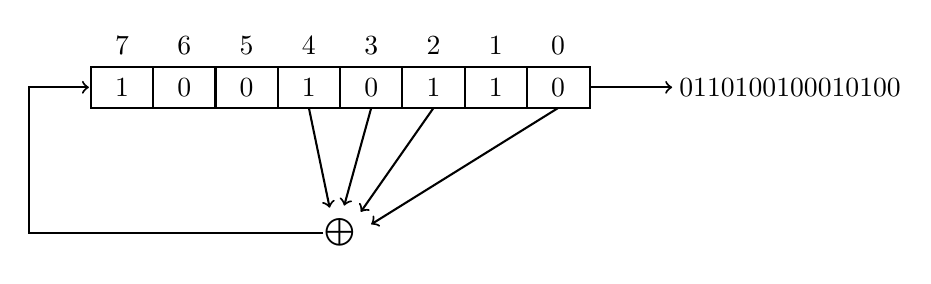
\begin{tikzpicture}[x=0.75pt,y=0.75pt,yscale=-1,xscale=1]

\draw   (60,20) -- (300.4,20) -- (300.4,40) -- (60,40) -- cycle ;

\draw    (90,20) -- (90,40) ;
\draw    (120,20) -- (120,40) ;
\draw    (150,20) -- (150,40) ;
\draw    (180,19.97) -- (180,40) ;
\draw    (210,20) -- (210,40) ;
\draw    (240,20) -- (240,40) ;
\draw    (270,20) -- (270,40) ;

\draw  [->]  (165,40) -- (175,88) ;
\draw  [->]  (195,40) -- (182,87) ;
\draw  [->]  (225,40) -- (190,90) ;
\draw  [->]  (285,40) -- (195,96) ;
\draw  [->]  (300,30) -- (340,30) ;
\draw  [->]  (172,100) -- (30,100) -- (30,30) -- (59,30) ;

\draw (75,30) node    {$1$};
\draw (105,30) node    {$0$};
\draw (135,30) node    {$0$};
\draw (165,30) node    {$1$};
\draw (195,30) node    {$0$};
\draw (225,30) node    {$1$};
\draw (255,30) node    {$1$};
\draw (285,30) node    {$0$};

\draw (75,10) node    {$7$};
\draw (105,10) node    {$6$};
\draw (135,10) node    {$5$};
\draw (165,10) node    {$4$};
\draw (195,10) node    {$3$};
\draw (225,10) node    {$2$};
\draw (255,10) node    {$1$};
\draw (285,10) node    {$0$};

\draw (180,100) node  [font=\large]  {$\bigoplus $};
\draw (342,30) node [anchor=west] [inner sep=0.75pt]    {$0110100100010100\dotsc $};

\end{tikzpicture}
	\caption{$8$比特的线性反馈移位寄存器$\{4,3,2,0\}$}
	\label{fig:3-10}
\end{figure}

\begin{snote}[来自 LSFR 的流密码。]
一个单一的 LFSR 作为 PRG 是完全不安全的,因为给定其输出的 $n$ 个连续比特,很容易就能计算出所有的后续比特。然而,使用一个非线性组件把几个 LFSR 组合起来,我们就有可能得到在某种程度上(弱)安全的 PRG。一种属于 eStream 组合的流密码 Trivium 就是这样构建出来的。

从 LFSR 构建流密码的一种方法是并行地运行几个 LFSR,并使用非线性操作组合它们的输出。接下来描述的 CSS 流密码使用整数域上的加法将两个 LFSR 组合起来。而被用于加密 GSM 手机流量的 A5/1 流密码组合了三个 LFSR 的输出。蓝牙 E0 流密码使用一个 $2$ 比特的有限状态机将四个 LFSR 组合起来。所有这些算法都已经被证明是不安全的,并且不应该再被使用。这是因为对于这些密码,恢复明文所需的时间远远少于对密钥空间进行穷举搜索的耗时。

另一种方法是只运行一个 LFSR,并对其内部状态进行非线性操作来产生输出。用于加密 3GPP 手机流量的 \texttt{snow} 3G 密码就是这样操作的。
\end{snote}

\begin{snote}[CSS 流密码。]
CSS 流密码是由图 \ref{fig:3-11} 所示的 PRG 构建的。该 PRG 的工作原理如下:

\vspace*{10pt}

\hspace*{5pt} 输入:种子 $s\in\{0,1\}^{40}$\\
\hspace*{26pt} 输出:$\ell$ 个比特

\vspace{5pt}

\hspace*{5pt} 令 $s=s_1\,\Vert\,s_2$,其中 $s_1\in\{0,1\}^{16}$,$s_2\in\{0,1\}^{24}$\\
\hspace*{26pt} 将 $1\,\Vert\,s_1$ 加载到一个 $17$ 比特的 LFSR 中\\
\hspace*{26pt} 将 $1\,\Vert\,s_2$ 加载到一个 $25$ 比特的 LFSR 中\\
\hspace*{26pt} 令 $c\leftarrow 0$ \quad\quad // \emph{进位}\\
\hspace*{26pt} 对于 $i=1,\dots,\ell$:\\
\hspace*{50pt} 将两个 LFSR 运行 $8$ 个周期,得到 $x_i,y_i\in\{0,1\}^8$\\
\hspace*{50pt} 将 $x_i$ 和 $y_i$ 视作 $\{0,\dots,255\}$ 中的两个整数\\
\hspace*{50pt} 输出 $z_i:=x_i+y_i+c\bmod 256$\\
\hspace*{50pt} 如果 $x_i+y_i>255$,则令 $c\leftarrow1$,否则令 $c\leftarrow0$ \quad\quad // \emph{进位}

\vspace*{10pt}

该 PRG 每次迭代输出一个字节。在 $s_1$ 和 $s_2$ 中预留的 $1$ 确保 LFSR 不会被初始化为全 $0$ 状态。两个 LFSR 的抽头是固定的。$17$ 比特的 LFSR 使用的是抽头 $\{14,0\}$,25比特的 LFSR 使用抽头 $\{12,4,3,0\}$。

我们展示的 CSS PRG 是 CSS 的一个小变体,它描述起来比较容易,但和真正的 CSS 具有同等的安全性。在真正的 CSS 中,对于 $17$ 比特的 LFSR,我们不是在初始种子中预置 $1$,而是在第 $9$ 比特的位置插入 $1$;而对于 $25$ 比特的 LFSR,是在第 $22$ 比特处插入 $1$。此外,真正的 CSS 会丢弃 $17$ 比特 LFSR 输出的第一个字节和 $25$ 比特 LFSR 输出的前两个字节。这两个问题都不会影响到接下来的分析。
\end{snote}

\begin{figure}
	\centering
	\tikzset{every picture/.style={line width=0.75pt}}      

\begin{tikzpicture}[x=0.75pt,y=0.75pt,yscale=-1,xscale=1]

\draw   (60,20) -- (300,20) -- (300,40) -- (60,40) -- cycle ;
\draw   (0,100) -- (300,100) -- (300,120) -- (0,120) -- cycle ;

\draw  [fill={rgb, 255:red, 255; green, 255; blue, 255 }  ,fill opacity=1 ][general shadow={fill={rgb, 255:red, 0; green, 0; blue, 0 }  ,shadow xshift=1.5pt,shadow yshift=-1.5pt, opacity=1 }] (280,60) -- (480,60) -- (480,80) -- (280,80) -- cycle ;

\draw  [->]  (300,30) -- (380,30) -- (380,60) ;
\draw  [->]  (300,110) -- (380,110) -- (380,82.5) ;
\draw  [->]  (480,70) -- (550,70) ;

\draw (180.2,30) node   [align=left] {$17$-bit LFSR};
\draw (150,110) node   [align=left] {$25$-bit LFSR};
\draw (380,70) node    {$x+y+c\bmod 256$};
\draw (340,113) node [anchor=north] [inner sep=0.75pt]   [align=left] {$8$ bits};
\draw (340,27) node [anchor=south] [inner sep=0.75pt]   [align=left] {$8$ bits};
\draw (382,45) node [anchor=west] [inner sep=0.75pt]    {$x$};
\draw (382,95) node [anchor=west] [inner sep=0.75pt]    {$y$};
\draw (515.17,73.4) node [anchor=north] [inner sep=0.75pt]    {$8$};

\end{tikzpicture}
	\caption{CSS流密码}
	\label{fig:3-11}
\end{figure}

\begin{snote}[CSS的不安全性。]
给定 PRG 的输出,通过对种子空间进行穷举搜索,我们显然可以在 $2^{40}$ 次计算内恢复秘密的种子。我们下面展示一种更快的攻击方法,它只需要进行 $2^{16}$ 次猜测。假设我们得到了 PRG 输出的前 $100$ 字节 $\bar{z}:=(z_1,z_2,\dots)$。该攻击基于以下观察:
\begin{quote}
令 $(x_1,x_2,x_3)$ 和 $(y_1,y_2,y_3)$ 分别为 $17$ 比特和 $25$ 比特 LFSR 输出的前 $3$ 字节。则有:
\[
(2^{16}x_3+2^8x_2+x_1)+(2^{16}y_3+2^8y_2+y_1)
\equiv(2^{16}z_3+2^8z_2+z_1)\;\;(\bmod\;2^{24})
\]
因此,一旦已知 $(z_1,z_2,z_3)$ 和 $(x_1,x_2,x_3)$,我们就很容易算出 $(y_1,y_2,y_3)$,进而很容易得到 $25$ 比特 LFSR 的初始状态 $s_2$。
\end{quote}
有了这个观察,攻击者就可以尝试 $s_1$ 的所有 $16$ 比特可能值,以此恢复种子 $s$。对于每个 $s_1$ 的猜测,攻击者计算出 $17$ 比特 LFSR 对应的输出 $(x_1,x_2,x_3)$。利用上面的观察,它就能够获得一个 $25$ 比特 LFSR 的候选种子 $s_2$。然后,为了确认 $\hat{s}:=s_1\Vert s_2$ 是否是正确的秘密种子,它使用种子 $\hat{s}$ 运行 PRG 的 $100$ 次迭代,并将输出的结果与给定的序列 $\bar{z}$ 进行比较。如果序列不匹配,就换一个 $s_1$ 重新进行计算。一旦攻击者找到了正确的 $s_1$,生成的序列就会与给定的 $\bar{z}$ 一致,在这种情况下,攻击者就得到了正确的秘密种子 $\hat{s}:=s_1\,\Vert\,s_2$。

我们上面的分析表明,对 $s_1$ 进行预计大概 $2^{15}$ 次猜测后,我们就可以恢复整个种子 $s$。这比单纯地进行 $2^{40}$ 次穷举搜索攻击要快得多。
\end{snote}
\section{练习}\label{sec:20-9}

\begin{exercise}\label{exer:20-1}
\end{exercise}

\begin{exercise}\label{exer:20-2}
\end{exercise}

\begin{exercise}\label{exer:20-3}
\end{exercise}

\begin{exercise}\label{exer:20-4}
\end{exercise}

\begin{exercise}\label{exer:20-5}
\end{exercise}

\begin{exercise}\label{exer:20-6}
\end{exercise}

\begin{exercise}\label{exer:20-7}
\end{exercise}

\begin{exercise}\label{exer:20-8}
\end{exercise}

\begin{exercise}\label{exer:20-9}
\end{exercise}

\begin{exercise}\label{exer:20-10}
\end{exercise}

\begin{exercise}\label{exer:20-11}
\end{exercise}

\begin{exercise}\label{exer:20-12}
\end{exercise}

\begin{exercise}\label{exer:20-13}
\end{exercise}

\begin{exercise}\label{exer:20-14}
\end{exercise}

\begin{exercise}\label{exer:20-15}
\end{exercise}

\begin{exercise}\label{exer:20-16}
\end{exercise}

\begin{exercise}\label{exer:20-17}
\end{exercise}

\begin{exercise}\label{exer:20-18}
\end{exercise}

\begin{exercise}\label{exer:20-19}
\end{exercise}

\begin{exercise}\label{exer:20-20}
\end{exercise}

\begin{exercise}\label{exer:20-21}
\end{exercise}

\begin{exercise}\label{exer:20-22}
\end{exercise}

\begin{exercise}\label{exer:20-23}
\end{exercise}

\begin{exercise}\label{exer:20-24}
\end{exercise}

\begin{exercise}\label{exer:20-25}
\end{exercise}

\begin{exercise}\label{exer:20-26}
\end{exercise}
